\chapter{The DNS traffic in Ireland}

The DNS traffic is an important consideration for building a DNS server. Irish TRR servers have to be capable to deal with the DNS traffic of national scale traffic in Ireland.
\\

Before understanding the DNS traffic in Ireland, it is necessary to understand the root servers first.
\\

Root servers are the highest level DNS servers \cite{dns_root_server_cloudflare}, there are 1097 instances in the root server system on 31 August 2020. They are divided into 13 root server zones, each zone has a representative letter, which are A, B, C, D, E, F, G, H, I, J, K, L and M \cite{root_server_wiki}. Those root server zones are managed by 12 organizations \cite{root_servers_org}, which are Verisign(It manages 2 root server zones), USC-ISI, Cogent Communications, University of Maryland, NASA Ames Research Center, Internet Systems Consortium, Defense Information Systems Agency, U.S. Army Research Lab, Netnod, RIPE NCC, ICANN and WIDE Project. Therefore, those 12 organizations have the information about DNS traffic.
\\


\begin{figure}[hbt!]  
    \centering
    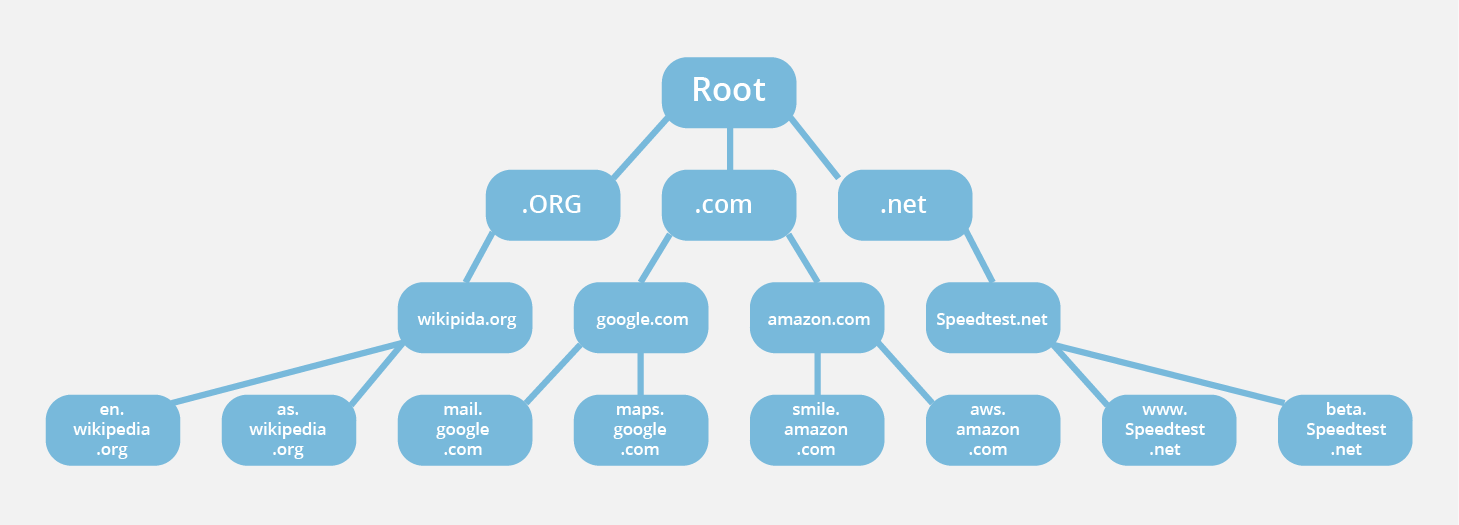
\includegraphics[width=0.8\textwidth]{figure/dns-root-server.png}
    \caption{\em The levels of authoritative DNS servers \cite{dns_root_server_cloudflare}}
    \label{fig:levels_authoritative_DNS_servers}
\end{figure}

\begin{figure}[hbt!]  
    \centering
    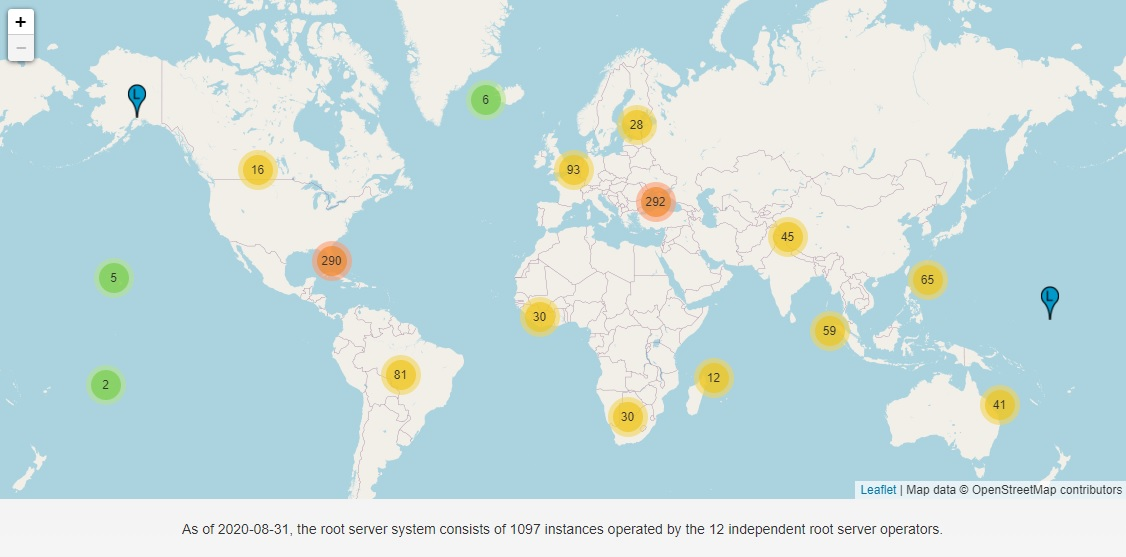
\includegraphics[width=0.8\textwidth]{figure/root-server-map-big.jpg}
    \caption{\em The root servers in the world \cite{root_servers_org} \label{fig:root_servers_in_the_world}}
\end{figure}

\begin{figure}[hbt!]  
    \centering
    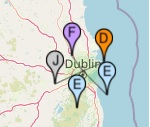
\includegraphics[width=0.4\textwidth]{figure/root-server-map-dublin.jpg}
    \caption{\em The root servers in Dublin \cite{root_servers_org} \label{fig:root_servers_dublin}}
\end{figure}

\begin{figure}[hbt!]  
    \centering
    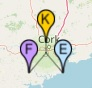
\includegraphics[width=0.4\textwidth]{figure/root-server-map-cork.jpg}
    \caption{\em The root servers in Cork \cite{root_servers_org} \label{fig:root_servers_cork}}
\end{figure}

In the map from Root-servers.org, there are 8 root servers in Ireland, 5 servers are in Dublin and 3 servers are in Cork. As for organizations, 3 servers belong to E-root(E zone, it is managed by NASA Ames Research Center), 2 servers belong to F-root(F zone, it is managed by Internet Systems Consortium). K-root(RIPE NCC), D-root(University of Maryland), J-root(Verisign) have 1 server respectively \cite{root_servers_org}.
\\

\begin{table}[hbt!]
    \centering
    \begin{tabular}{|c|c|c|}
        \hline
          Zone & Operator & Number in Ireland\\    
        \hline
        A & Verisign & 0 \\
        \hline
        B & USC-ISI & 0\\
        \hline
        C & Cogent Communications & 0 \\
        \hline
        D & University of Maryland & 1\\
        \hline
        E & NASA Ames Research Center & 3\\
        \hline
        F & Internet Systems Consortium & 2\\
        \hline
        G & Defense Information Systems Agency & 0\\
        \hline
        H & U.S. Army Research Lab & 0\\
        \hline
        I & Netnod & 0\\
        \hline
        J & Verisign & 1\\
        \hline
        K & RIPE NCC & 1\\
        \hline
        L & ICANN & 0\\
        \hline
        M & WIDE Project & 0\\
        \hline
    \end{tabular}
    \caption{The list of root server zones \cite{root_servers_org}}
    \label{tab:root_server_zone_list}
\end{table}

The problem is the information those organizations provided on Internet is limited. There is no statistic data of DNS queries in Ireland on their website.
\\

Next, the recursive structure of DNS servers has to be figured out. There are two kinds of DNS servers, the first kind of DNS server is recursive DNS server, it could be private or public, but those recursive DNS servers are not controlled by the organizations mentioned above. When users send queries to DNS servers, the queries will arrive recursive DNS servers first, if recursive DNS servers have matched IP addresses in their caches, then they can respond IP addresses to users directly. 
\\

The second DNS server is authoritative DNS server, they store the IP addresses of websites. Moreover, they are hierarchical, the highest one is root server. The levels of authoritative DNS servers are shown in Fig.~\ref{tab:Authoritative_DNS_server_levels}. If recursive DNS servers do not have matched IP addresses, they will ask authoritative DNS server for IP addresses and store it in their cache \cite{Authoritative_vs_Recursive_DNS_server}.
\\

Thus, the recursive structure of DNS server causes another problem, it is very hard to collect the records about all DNS queries, because there are numerous recursive DNS servers and they are managed by many organizations \cite{Authoritative_and_recursive_DNS}, hence, the operators of root servers do not have their data.
\\

However, it is not necessary to know the total number of DNS queries in Ireland, because the target in this research is to understand what the performance should a TTR server possess in Ireland. The number of DNS queries a root server may receive can help us to evaluate the required performance for a TTR server in Ireland.
\\

In this paper, the researcher designs some methods to estimate the traffic a DNS server would have in Ireland by using the traffic in root servers.
\\

Method 1 is using the data on Akamai.com to estimate the DNS traffic \cite{overall_DNS_traffic_trends}.
\\

In website Akamai.com, it collects the DNS traffic from 9 root server zones(B, C, D, E, F, I, K, L, M), but the DNS traffic is worldwide, it does not provide the data in national scale or city scale on the website.
\\

Even though there is no national scale data on Akamai.com, but the worldwide data can be used to estimate the Irish DNS traffic.
\\

In a report from Central Statistics Office of Ireland, it showed that there were 89\% of Irish households have the internet at home in 2018 \cite{Irish_households_with_internet}. From the growth of households with the internet, the percentage is probably 90\% in 2020. There were about 4.57 billion internet users in the world in July 2020 \cite{Global_digital_population_July_2020}. The population in Ireland was around 4.944 million in August 2020 \cite{Ireland_population}. Hence, the Irish Internet users may be about 4.113 million, it was approximately 0.09\% of internet users in the whole world.
\\

According to the data from Akamai.com \cite{overall_DNS_traffic_trends}, the overall DNS traffic in the world was about 7 Trillion transactions (Requests and responses) in June 2020. 
Then, 0.09\% of DNS traffic in the world could be Irish DNS traffic, which is around 6.3 billion DNS transactions for one month in Ireland. On average, it could be 210 DNS million transactions in a day in Ireland.
\\

\begin{figure}[hbt!]  
    \centering
    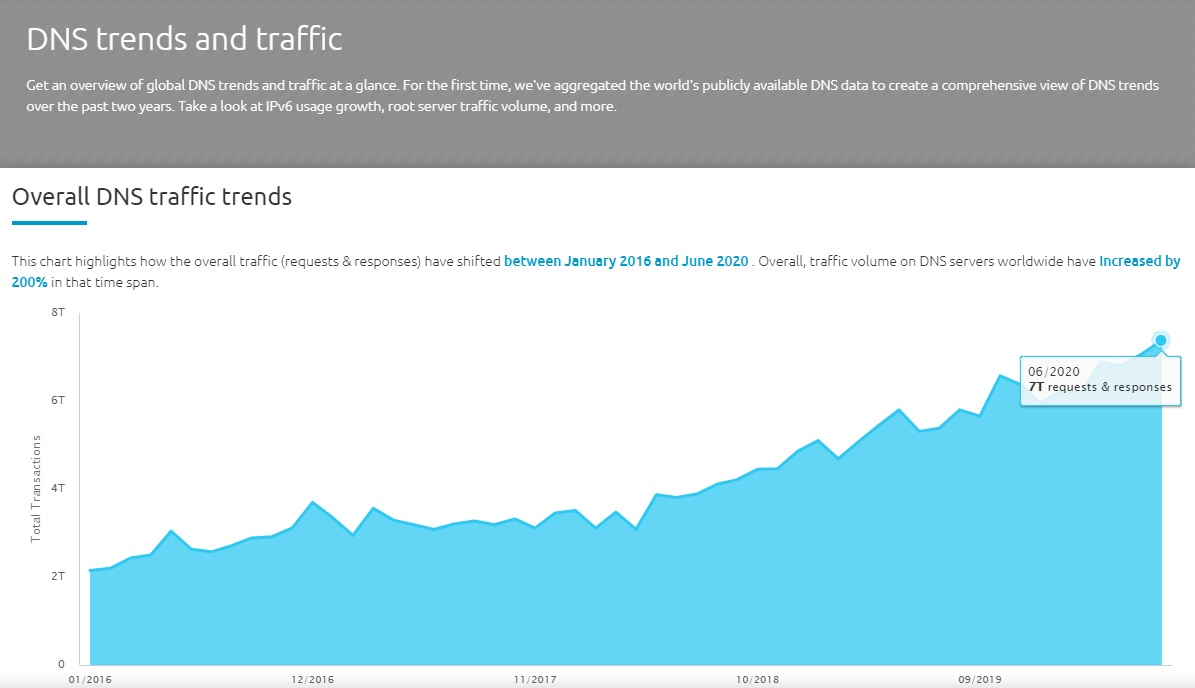
\includegraphics[width=0.8\textwidth]{figure/Overall DNS traffic trends.jpg}
    \caption{\em The trend of DNS traffic in the world \cite{overall_DNS_traffic_trends} \label{fig:trend_DNS_traffic}}
\end{figure}

\begin{table}[hbt!]
    \centering
    \begin{tabular}{|c|c|c|c|}
        \hline
         Month & IPv4 & IPv6 & Total\\
        \hline
         06/2020 & 6T & 1T & 7T \\
        \hline
        01/2020 & 5T & 969B & 6T\\
        \hline
        07/2019 & 4T & 919B & 5T \\
        \hline
        01/2019 & 4T & 848B & 5T \\
        \hline
        07/2018 & 3T & 564B & 4T \\
        \hline
        01/2018 & 3T & 426B & 4T \\
        \hline
        07/2017 & 3T & 371B & 3T \\
        \hline
        01/2017 & 3T & 363B & 3T \\
        \hline
        07/2016 & 2T & 248B & 3T \\
        \hline
        01/2016 & 2T & 171B & 2T \\
        \hline
    \end{tabular}
    \caption{Overall DNS traffic trends(Unit:Transactions) \cite{overall_DNS_traffic_trends}}
    \label{tab:DNS_traffic_trends}
\end{table}

However, internet traffic is changeable in different hours, it is necessary to understand when are the rush hours. For example, the internet rush hours are usually between 7 pm and 11 pm in UK \cite{Avoiding_the_internet_rush_hour}. In Sao Paulo, the internet rush hours are between 8 pm and 11 pm \cite{Brazil_internet_rush_hour}. In USA, it is 8 pm to 10 pm \cite{Measuring_broadband_america}. In Berlin, the rush hours are 8 pm to 11 pm \cite{Berlin_internet_traffic}. In Amsterdam, it is from 8 pm to 11 pm as well \cite{Amsterdam_internet_traffic}.
\\

\begin{figure}[hbt!]
    \centering
    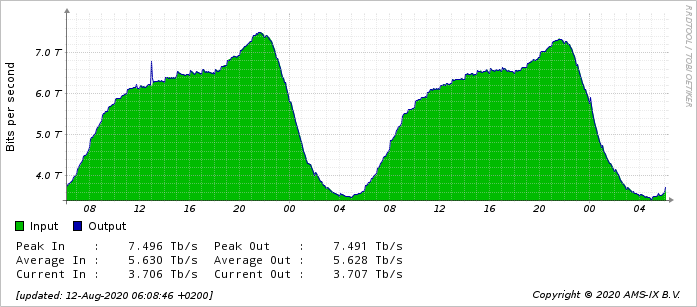
\includegraphics[width=0.8\textwidth]{figure/amsterdam-day.png}
    \caption{\em The internet traffic in a day (Amsterdam) \cite{Amsterdam_internet_traffic} \label{fig:internet_traffic_day_Amsterdam}}
\end{figure}

\begin{figure}[hbt!]    
    \centering
    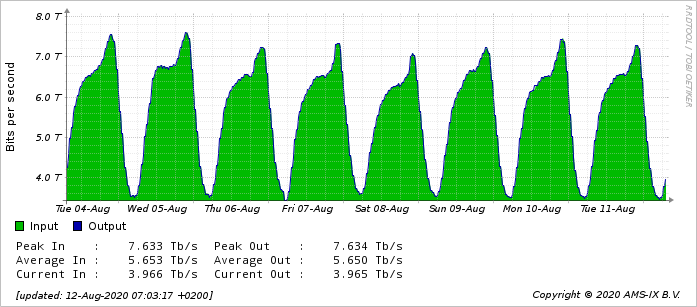
\includegraphics[width=0.8\textwidth]{figure/amsterdam-week.png}
    \caption{\em The internet traffic in a week (Amsterdam) \cite{Amsterdam_internet_traffic} \label{fig:internet_traffic_week_Amsterdam}}
\end{figure}

\begin{figure}[hbt!]  
    \centering
    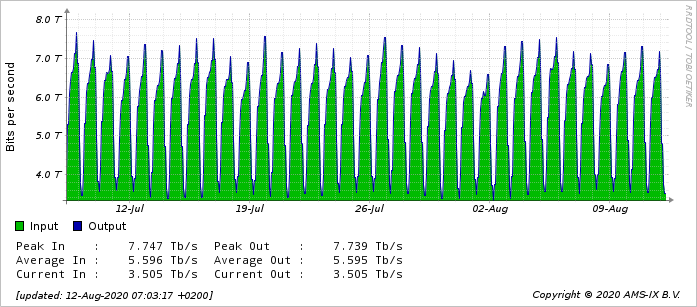
\includegraphics[width=0.8\textwidth]{figure/amsterdam-month.png}
    \caption{\em The internet traffic in a month (Amsterdam) \cite{Amsterdam_internet_traffic} \label{fig:internet_traffic_month_Amsterdam}}
\end{figure}

\begin{figure}[hbt!]
    \centering
    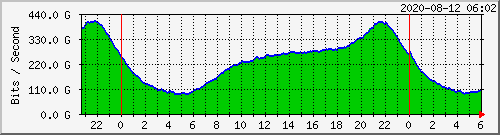
\includegraphics[width=0.8\textwidth]{figure/berlin-day.png}
    \caption{\em The internet traffic in a day (Berlin) \cite{Amsterdam_internet_traffic} \label{fig:internet_traffic_day_Berlin}}
\end{figure}

\begin{figure}[hbt!]
    \centering
    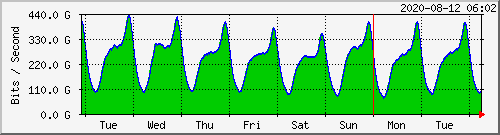
\includegraphics[width=0.8\textwidth]{figure/berlin-week.png}
    \caption{\em The internet traffic in a week (Berlin) \cite{Amsterdam_internet_traffic} \label{fig:internet_traffic_week_Berlin}}
\end{figure}

\begin{figure}[hbt!]
    \centering
    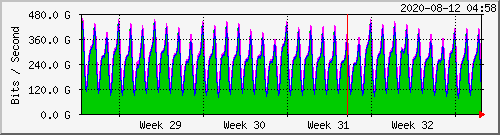
\includegraphics[width=0.8\textwidth]{figure/berlin-month.png}
    \caption{\em The internet traffic in a month (Berlin) \cite{Amsterdam_internet_traffic} \label{fig:internet_traffic_month_Berlin}}
\end{figure}

All the reports in different countries or cities revealed that internet rush hours are from 8 pm to 11 pm, the distributions are pretty similar. Therefore, Irish internet rush hours could be assumed as from 8 pm to 11 pm as well. 
\\

As for the comparison in different days in a week, from Monday to Sunday, the change is not obvious. About the days in a month, from the begin to the end of a month, there is no huge difference as well.
\\

Taking the data in Amsterdam to estimate the percentage of usage in each hour, the result is shown in TABLE ~\ref{tab:table_amsterdam}.
\\

\begin{table}[hbt!]
    \centering
    \begin{tabular}{|c|c|c|}
        \hline
         Hour(24) & Trillion bit/s & Percentage\\
        \hline
        0 & 5.8 & 4.3\% \\
        \hline
        1 & 4.8 & 3.56\% \\
        \hline
        2 & 4 & 2.96\% \\
        \hline
        3 & 3.7 & 2.74\% \\
        \hline
        4 & 3.6 & 2.67\% \\
        \hline
        5 & 3.5 & 2.59\% \\
        \hline
        6 & 3.6 & 2.67\%  \\
        \hline
        7 & 4 & 2.96\%  \\
        \hline
        8 & 4.8 & 3.56\%  \\
        \hline
        9 & 5.4 & 4\%  \\
        \hline
        10 & 5.8 & 4.3\%  \\
        \hline
        11 & 6 & 4.44\% \\
        \hline
        12 & 6.2 & 4.59\%  \\
        \hline
        13 & 6.4 & 4.74\%  \\
        \hline
        14 & 6.4 & 4.74\%  \\
        \hline
        15 & 6.6 & 4.89\%  \\
        \hline
        16 & 6.6 & 4.89\%  \\
        \hline
        17 & 6.6 & 4.89\%  \\
        \hline
        18 & 6.5 & 4.81\%  \\
        \hline
        19 & 6.7 & 4.96\%  \\
        \hline
        20 & 6.9 & 5.11\%  \\
        \hline
        21 & 7.2 & 5.33\%  \\
        \hline
        22 & 7.2 & 5.33\%  \\
        \hline
        23 & 6.7 & 4.96\% \\
        \hline
        Total & 135 & 100\%  \\
        \hline
    \end{tabular}
    \caption{Internet traffic and its percentage in each hour in a day in Amsterdam \cite{Amsterdam_internet_traffic}}
    \label{tab:table_amsterdam}
\end{table}

After that, using the percentage to multiply the estimated number of daily DNS transactions in Ireland, which is 210 million, then the result is sown in TABLE ~\ref{tab:table_dns_Ireland}. The 2 busiest hours are 9 PM and 10 PM, the number of DNS transactions could be  11.2 million in an hour.
\\

\begin{table}[hbt!]
    \centering
    \begin{tabular}{|c|c|c|}
        \hline
         Hour(24) & Percentage & Million transactions\\
        \hline
        0 & 4.3\% & 9.02 \\
        \hline
        1 & 3.56\% & 7.47 \\
        \hline
        2 & 2.96\% & 6.22 \\
        \hline
        3 & 2.74\% & 5.76 \\
        \hline
        4 & 2.67\% & 5.6 \\
        \hline
        5 & 2.59\% & 5.44 \\
        \hline
        6 & 2.67\% & 5.6  \\
        \hline
        7 & 2.96\% & 6.22  \\
        \hline
        8 & 3.56\% & 7.47  \\
        \hline
        9 & 4\% & 8.4  \\
        \hline
        10 & 4.3\% & 9.02  \\
        \hline
        11 & 4.44\% & 9.33 \\
        \hline
        12 & 4.59\% & 9.64  \\
        \hline
        13 & 4.74\% & 9.96 \\
        \hline
        14 & 4.74\% & 9.96 \\
        \hline
        15 & 4.89\% & 10.27 \\
        \hline
        16 & 4.89\% & 10.27 \\
        \hline
        17 & 4.89\% & 10.27 \\
        \hline
        18 & 4.81\% & 10.11 \\
        \hline
        19 & 4.96\% & 10.42 \\
        \hline
        20 & 5.11\% & 10.73 \\
        \hline
        21 & 5.33\% & 11.2 \\
        \hline
        22 & 5.33\% & 11.2 \\
        \hline
        23 & 4.96\% & 10.42 \\
        \hline
        Total & 100\% & 210  \\
        \hline
    \end{tabular}
    \caption{Using the daily distribution of Internet traffic of Amsterdam to estimate the DNS traffic in Ireland \cite{Amsterdam_internet_traffic}}
    \label{tab:table_dns_Ireland}
\end{table}

However, the data from Akamai.com does not include A, G, H and J root server zones. Thus, the number of transactions in rush hours should be higher than 11.2 million.
\\

The numbers of transactions in every root server zone are very different, therefore it is hard to estimate the numbers in A, G, H and J root server zones. If assume that the average number of A, G, H and J is close to the average number of B, C, D, E, F, I, K, L, M, then the estimated number of transactions in all root servers in rush hours could be 11.2/9X13=16.18 million.
\\

If convert it into a second, the number of DNS transactions could be 4,494 per second during the rush hour (16.18(million per hour)/60(minutes)/60(seconds)).
\\

Method 2 is using the data from ICANN to estimate DNS traffic. 
\\

ICANN (Internet Corporation for Assigned Names and Numbers) is the one of 12 organizations which are responsible for managing DNS root servers, the servers it manages are L-root servers. Unlike other 11 organizations, ICANN provides a website to display real-time DNS traffic, that is Stats.dns.icann.org \cite{stats_dns_icann_org}.
\\

The problem is ICANN does not have root servers in Ireland. Moreover, those data is only from ICANN, it does not include the data from other root server zones.
\\

Thus, here chose a city which has a similar population to Ireland to estimate the DNS traffic. Melbourne should be a ideal sample. The population in Melbourne is about 5 million in 2019 \cite{Melbourne_wiki}, which is close to the population in Ireland (4.9 million). Moreover, Melbourne is isolated, there is no big city near Melbourne,therefore the network connection may be similar to a country.
\\

\begin{figure}[hbt!]
    \centering
    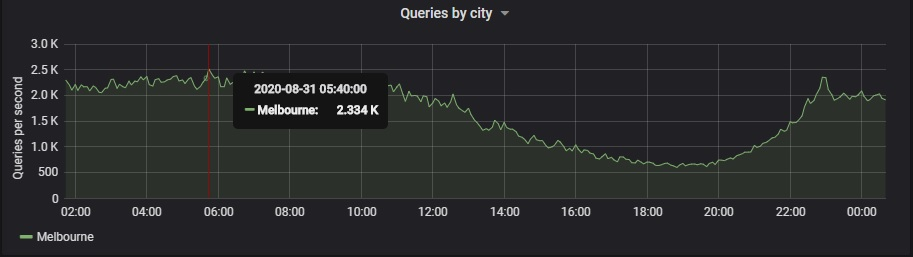
\includegraphics[width=0.8\textwidth]{figure/melbourne.jpg}
    \caption{\em The number of queries per second in a root server in Melbourne \cite{stats_dns_icann_org} }
    \label{tab:figure_melbourne}
\end{figure}

From the data in Fig.~\ref{tab:figure_melbourne}, the highest value in a day is 2,334 per second, which was occurred at 05:40 UTC(19:40 in Melbourne).
\\

\begin{figure}[hbt!]  
    \centering
    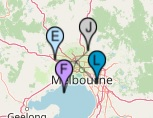
\includegraphics[width=0.4\textwidth]{figure/root-server-map-melbourne.jpg}
    \caption{\em The root servers in Melbourne \cite{root_servers_org} \label{fig:root_servers_Melbourne}}
\end{figure}

However, the data is only from a root server which is managed by ICANN, there are four root servers in Melbourne, the DNS traffic in other 3 root servers are not provided. Assume the average traffic in other 3 root servers is close to the root server managed by ICANN, the whole DNS traffic in Melbourne could be 9,336 per second(2,334X4). Next, adjust the traffic to accord the population of Ireland, the DNS traffic could be 9,149 per second during the rush hour(9,336/5X4.9).
\\

The comparison between method 1 and method 2 is shown in TABLE ~\ref{tab:estimation_comparison}.
\\


\begin{table}[hbt!]
    \centering
    \begin{tabular}{|p{2cm}|p{2.5cm}|p{2.5cm}|}
        \hline
          & Method 1 & Method 2\\    
        \hline
        Source & Akamai.com & ICANN \\
        \hline
         Queries per second in rush hours & 4,494 & 9,149\\
        \hline
         Drawback 1 & No Irish data & No Irish data \\
        \hline
         Drawback 2 & Only monthly data & The data is only from L-root\\
        \hline
    \end{tabular}
    \caption{The comparison between 2 methods for the estimation of the DNS traffic in Ireland}
    \label{tab:estimation_comparison}
\end{table}

	\section{Section 1.1}

	...
